\section{演化樹分析 (Agreement)}

\subsection{問題描述}

彼得是一位生物學家。有次他在兩筆資料中分析同一群現存物種集合
\(\Sigma = \{1, 2, \ldots, n\}\)
間的演化關係,卻得到了不太一樣的演化樹,想知道這兩棵演化樹的類似程度。

一棵演化樹 \(T\) 是一棵無向無根樹 (undirected, unrooted
tree),其中葉節點為現存物種
\(1, 2, \ldots, n\),其他節點則為已滅絕物種。設 \(v \in V(T)\),我們用
\(\deg(v)\) 來表示與節點 \(v\)
相鄰的節點個數。在一棵演化樹中,每個代表已滅絕物種的節點 \(v\) 均有
\(\deg(v) \ge 3\)。對於一個現存物種的子集合
\(X \subseteq \Sigma\),我們用 \(T\{X\}\) 來代表 \(X\) 中的現存物種在
\(T\) 上的演化關係所形成的「演化子樹」,建構方式如下:

\begin{enumerate}
\def\labelenumi{\arabic{enumi}.}
\tightlist
\item
  對所有 \(X\) 中的任兩點,標記其在 \(T\) 上的簡單路徑,並將所有不在
  \(X\) 且未被標記的點刪除以得到 \(T'\)。
\item
  從 \(T'\) 中不斷刪除滿足 \(\deg(v) = 2\) 的非葉節點 \(v\) 以得到
  \(T\{X\}\):將與 \(v\) 連結的兩條邊合併成一條,並移除 \(v\)。
\end{enumerate}

\noindent 以下圖的演化樹 \(T\) 為例。\(T\) 裡的現存物種集合為
\(\Sigma = \{1, 2, 3, 4, 5\}\),若取 \(X = \{3, 4, 5\}\),則經步驟 \(1\)
後會得到 \(T'\),再經過步驟 \(2\) 後會得到 \(T\{X\}\)。注意當
\(X = \emptyset\) 時,根據定義我們有 \(T\{X\} = \emptyset\)。

\begin{minipage}{0.33\textwidth}
  \begin{figure}[H]
    \centering
    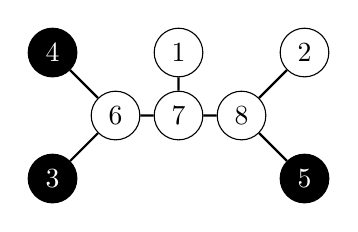
\begin{tikzpicture}[scale=0.8]
      \def \Nodes{
        1/2/2/white/black,
        2/4/2/white/black,
        3/0/0/black/white,
        4/0/2/black/white,
        5/4/0/black/white,
        6/1/1/white/black,
        7/2/1/white/black,
        8/3/1/white/black}
      \def \Edges{
        1/7,
        2/8,
        3/6,
        4/6,
        5/8,
        6/7,
        7/8}
      \foreach \id / \x / \y / \c / \d in \Nodes{
        \node[draw,circle,fill=\c] (\id) at (\x, \y) {\textcolor{\d}{\id}};
      }
      \foreach \x / \y in \Edges{
        \path[draw,-,thick] (\x) -- (\y);
      }
    \end{tikzpicture}
    \caption{$T$}
  \end{figure}
\end{minipage}
\begin{minipage}{0.33\textwidth}
  \begin{figure}[H]
    \centering
    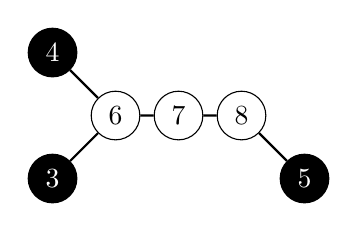
\begin{tikzpicture}[scale=0.8]
      \def \Nodes{
        3/0/0/black/white,
        4/0/2/black/white,
        5/4/0/black/white,
        6/1/1/white/black,
        7/2/1/white/black,
        8/3/1/white/black}
      \def \Edges{
        3/6,
        4/6,
        5/8,
        6/7,
        7/8}
      \foreach \id / \x / \y / \c / \d in \Nodes{
        \node[draw,circle,fill=\c] (\id) at (\x, \y) {\textcolor{\d}{\id}};
      }
      \foreach \x / \y in \Edges{
        \path[draw,-,thick] (\x) -- (\y);
      }
    \end{tikzpicture}
    \caption{$T'$}
  \end{figure}
\end{minipage}
\begin{minipage}{0.33\textwidth}
  \begin{figure}[H]
    \centering
    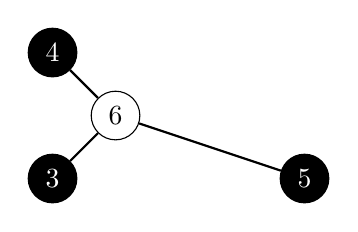
\begin{tikzpicture}[scale=0.8]
      \def \Nodes{
        3/0/0/black/white,
        4/0/2/black/white,
        5/4/0/black/white,
        6/1/1/white/black}
      \def \Edges{
        3/6,
        4/6,
        5/6}
      \foreach \id / \x / \y / \c / \d in \Nodes{
        \node[draw,circle,fill=\c] (\id) at (\x, \y) {\textcolor{\d}{\id}};
      }
      \foreach \x / \y in \Edges{
        \path[draw,-,thick] (\x) -- (\y);
      }
    \end{tikzpicture}
    \caption{$T\{X\}$}
  \end{figure}
\end{minipage}

從一棵演化樹 \(T\) 中移除大小為 \(k \ge 0\) 的任意邊集合 \(K\),可以得到
\(k+1\) 棵子樹 \(T^{(1)}, T^{(2)}, \ldots, T^{(k+1)}\),其中每棵子樹
\(T^{(i)}\) 上的物種在 \(T\)
中的演化關係都會構成一棵\textbf{演化子樹},我們稱它們為從 \(T\) 中移除
\(K\) 所導出的\textbf{演化森林}。注意我們有

\begin{enumerate}
\def\labelenumi{\arabic{enumi}.}
\tightlist
\item
  \(T\) 自身為移除 \(\emptyset\) 後導出的演化森林。
\item
  若一棵子樹 \(T^{(i)}\) 上沒有任何現存物種,對應的演化子樹為空。
\end{enumerate}

\noindent 以上圖中的 \(T\) 為例,移除
\(K = \{(1, 7), (7, 8), (2, 8), (5, 8)\}\) 四條邊可以得到五棵子樹
\(T^{(1)}, T^{(2)}, \ldots, T^{(5)}\),接著導出演化森林:

\newpage

\begin{minipage}{0.33\textwidth}
  \begin{figure}[H]
    \centering
    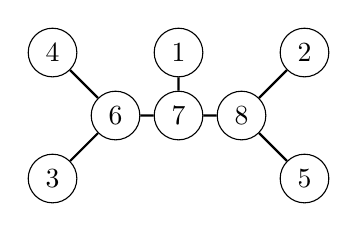
\begin{tikzpicture}[scale=0.8]
      \def \Nodes{
        1/2/2,
        2/4/2,
        3/0/0,
        4/0/2,
        5/4/0,
        6/1/1,
        7/2/1,
        8/3/1}
      \def \Edges{
        1/7,
        2/8,
        3/6,
        4/6,
        5/8,
        6/7,
        7/8}
      \foreach \id / \x / \y in \Nodes{
        \node[draw,circle] (\id) at (\x, \y) {\id};
      }
      \foreach \x / \y in \Edges{
        \path[draw,-,thick] (\x) -- (\y);
      }
    \end{tikzpicture}
    \caption{移除 $K$ 前}
  \end{figure}
\end{minipage}
\begin{minipage}{0.33\textwidth}
  \begin{figure}[H]
    \centering
    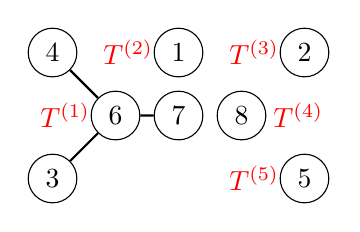
\begin{tikzpicture}[scale=0.8]
      \def \Nodes{
        1/2/2,
        2/4/2,
        3/0/0,
        4/0/2,
        5/4/0,
        6/1/1,
        7/2/1,
        8/3/1}
      \def \Edges{
        3/6,
        4/6,
        6/7}
      \foreach \id / \x / \y in \Nodes{
        \node[draw,circle] (\id) at (\x, \y) {\id};
      }
      \node[red] at (0.2, 1){$T^{(1)}$};
      \node[red] at (1.2, 2){$T^{(2)}$};
      \node[red] at (3.2, 2){$T^{(3)}$};
      \node[red] at (3.9, 1){$T^{(4)}$};
      \node[red] at (3.2, 0){$T^{(5)}$};
      \foreach \x / \y in \Edges{
        \path[draw,-,thick] (\x) -- (\y);
      }
    \end{tikzpicture}
    \caption{移除 $K$ 後}
  \end{figure}
\end{minipage}
\begin{minipage}{0.33\textwidth}
  \begin{figure}[H]
    \centering
    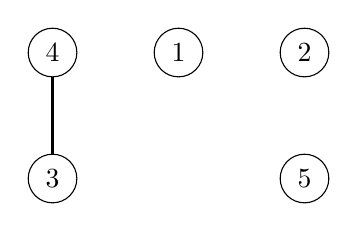
\begin{tikzpicture}[scale=0.8]
      \def \Nodes{
        1/2/2,
        2/4/2,
        3/0/0,
        4/0/2,
        5/4/0}
      \def \Edges{
        3/4}
      \foreach \id / \x / \y in \Nodes{
        \node[draw,circle] (\id) at (\x, \y) {\id};
      }
      \foreach \x / \y in \Edges{
        \path[draw,-,thick] (\x) -- (\y);
      }
    \end{tikzpicture}
    \caption{導出的演化森林}
  \end{figure}
\end{minipage}

比較兩座現存物種相同的演化森林時,我們只關注現存物種間的關係,因此已滅絕物種(即非葉節點)的編號並不重要。設
\(F_1\) 與 \(F_2\)
為兩座現存物種相同的演化森林,若移除它們的非葉節點編號後變得完全相同,我們就稱
\(F_1\) 與 \(F_2\) 類似。更精確地說,我們稱 \(F_1\) 與 \(F_2\)
類似,若且唯若存在某個一對一函數 \(\Phi: V(F_1) \to V(F_2)\),滿足

\begin{enumerate}
\def\labelenumi{\arabic{enumi}.}
\tightlist
\item
  對任意 \(u \in \Sigma = \{1, 2, \ldots, n\}\),我們有
  \(\Phi(u) = u\)。
\item
  對任意 \(u, v \in V(F_1)\),我們有
  \[(u, v) \in E(F_1) \iff (\Phi(u), \Phi(v)) \in E(F_2).\]
\end{enumerate}

以下圖為例,如果將 \(T_1, T_2, T_3\) 的非葉節點編號都移除,會發現
\(T_1\) 與 \(T_2\) 不類似,而 \(T_2\) 與 \(T_3\) 類似。

\begin{minipage}{0.33\textwidth}
  \begin{figure}[H]
    \centering
    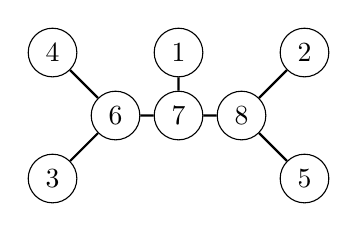
\begin{tikzpicture}[scale=0.8]
      \def \Nodes{
        1/2/2,
        2/4/2,
        3/0/0,
        4/0/2,
        5/4/0,
        6/1/1,
        7/2/1,
        8/3/1}
      \def \Edges{
        1/7,
        2/8,
        3/6,
        4/6,
        5/8,
        6/7,
        7/8}
      \foreach \id / \x / \y in \Nodes{
        \node[draw,circle] (\id) at (\x, \y) {\id};
      }
      \foreach \x / \y in \Edges{
        \path[draw,-,thick] (\x) -- (\y);
      }
    \end{tikzpicture}
    \caption{$T_1$}
  \end{figure}
\end{minipage}
\begin{minipage}{0.33\textwidth}
  \begin{figure}[H]
    \centering
    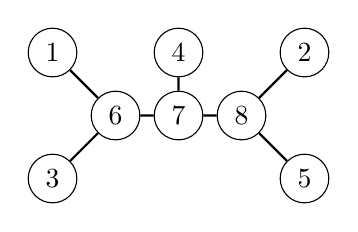
\begin{tikzpicture}[scale=0.8]
      \def \Nodes{
        1/0/2,
        2/4/2,
        3/0/0,
        4/2/2,
        5/4/0,
        6/1/1,
        7/2/1,
        8/3/1}
      \def \Edges{
        1/6,
        2/8,
        3/6,
        4/7,
        5/8,
        6/7,
        7/8}
      \foreach \id / \x / \y in \Nodes{
        \node[draw,circle] (\id) at (\x, \y) {\id};
      }
      \foreach \x / \y in \Edges{
        \path[draw,-,thick] (\x) -- (\y);
      }
    \end{tikzpicture}
    \caption{$T_2$}
  \end{figure}
\end{minipage}
\begin{minipage}{0.33\textwidth}
  \begin{figure}[H]
    \centering
    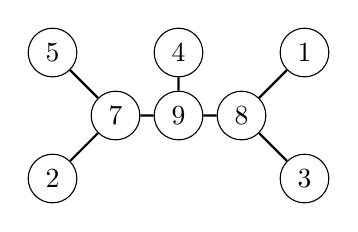
\begin{tikzpicture}[scale=0.8]
      \def \Nodes{
        1/4/2,
        2/0/0,
        3/4/0,
        4/2/2,
        5/0/2,
        7/1/1,
        9/2/1,
        8/3/1}
      \def \Edges{
        1/8,
        2/7,
        3/8,
        4/9,
        5/7,
        7/9,
        9/8}
      \foreach \id / \x / \y in \Nodes{
        \node[draw,circle] (\id) at (\x, \y) {\id};
      }
      \foreach \x / \y in \Edges{
        \path[draw,-,thick] (\x) -- (\y);
      }
    \end{tikzpicture}
    \caption{$T_3$}
  \end{figure}
\end{minipage}

設 \(T_1\) 與 \(T_2\) 為現存物種相同的兩棵演化樹。若存在從 \(T_1\) 與
\(T_2\) 中各刪除 \(k\) 條邊的方法,使得兩者導出的演化森林類似,則稱
\(T_1\) 與 \(T_2\) 的差異不大於 \(k\),而滿足此條件的最小整數 \(k^*\)
稱為 \(T_1\) 與 \(T_2\) 的\textbf{差異數}。如上圖中 \(T_2\) 與 \(T_3\)
的差異數為 \(0\),而 \(T_1\) 與 \(T_2\) 的差異數為 \(1\)。

\begin{minipage}{0.49\textwidth}
  \begin{figure}[H]
    \centering
    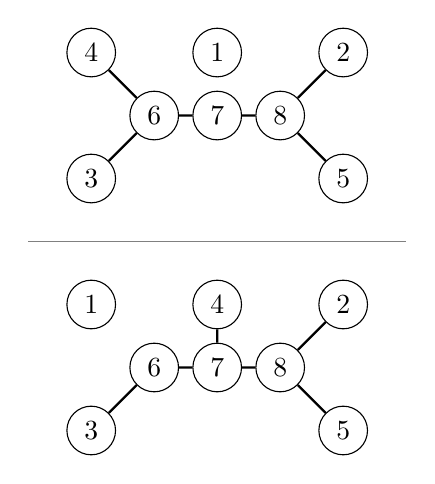
\begin{tikzpicture}[scale=0.8]
      \def \Nodes{
        1/2/6/1,
        2/4/6/2,
        3/0/4/3,
        4/0/6/4,
        5/4/4/5,
        6/1/5/6,
        7/2/5/7,
        8/3/5/8,
        a/0/2/1,
        b/4/2/2,
        c/0/0/3,
        d/2/2/4,
        e/4/0/5,
        f/1/1/6,
        g/2/1/7,
        h/3/1/8}
      \def \Edges{
        2/8,
        3/6,
        4/6,
        5/8,
        6/7,
        7/8,
        b/h,
        c/f,
        d/g,
        e/h,
        f/g,
        g/h}
      \foreach \id / \x / \y / \lb in \Nodes{
        \node[draw,circle] (\id) at (\x, \y) {\lb};
      }
      \foreach \x / \y in \Edges{
        \path[draw,-,thick] (\x) -- (\y);
      }
      \draw[color=gray] (-1, 3) -- (5, 3);
    \end{tikzpicture}
    \caption{從 $T_1$ 與 $T_2$ 各刪除 $1$ 條邊}
  \end{figure}
\end{minipage}
\begin{minipage}{0.49\textwidth}
  \begin{figure}[H]
    \centering
    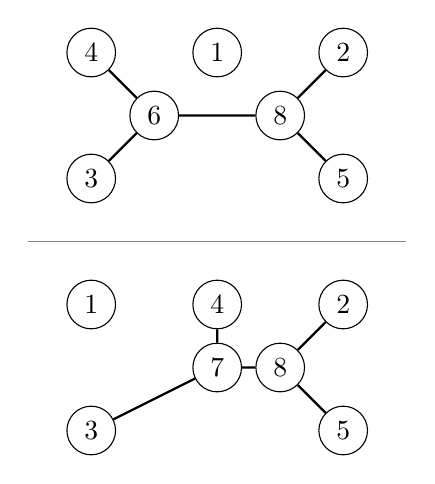
\begin{tikzpicture}[scale=0.8]
      \def \Nodes{
        1/2/6/1,
        2/4/6/2,
        3/0/4/3,
        4/0/6/4,
        5/4/4/5,
        6/1/5/6,
        8/3/5/8,
        a/0/2/1,
        b/4/2/2,
        c/0/0/3,
        d/2/2/4,
        e/4/0/5,
        g/2/1/7,
        h/3/1/8}
      \def \Edges{
        2/8,
        3/6,
        4/6,
        5/8,
        6/8,
        b/h,
        c/g,
        d/g,
        e/h,
        g/h}
      \foreach \id / \x / \y / \lb in \Nodes{
        \node[draw,circle] (\id) at (\x, \y) {\lb};
      }
      \foreach \x / \y in \Edges{
        \path[draw,-,thick] (\x) -- (\y);
      }
      \draw[color=gray] (-1, 3) -- (5, 3);
    \end{tikzpicture}
    \caption{導出了類似的演化森林}
  \end{figure}
\end{minipage}

設從 \(T_1\) 與 \(T_2\) 中刪除的邊集合分別為 \(K_1\) 與
\(K_2\),兩種刪除方法被視為不同若且唯若 \(K_1\) 不同或 \(K_2\)
不同。現給定兩棵物種集合均為 \(\Sigma\) 的演化樹 \(T_1, T_2\)
以及一個整數上限 \(k\),彼得想知道它們的差異數 \(k^*\) 是否不大於
\(k\);如果 \(1 \le k^* \le k\),彼得也想知道有多少種從 \(T_1\) 和
\(T_2\) 中各刪除 \(k^*\) 條邊的方法,可以使它們導出類似的演化森林。

\subsection{輸入格式}

\begin{format}
\f{
$n$ $m_1$ $m_2$ $k$
$u_1$ $v_1$
$u_2$ $v_2$
$\vdots$
$u_{n+m_1-1}$ $v_{n+m_1-1}$
$u_1'$ $v_1'$
$u_2'$ $v_2'$
$\vdots$
$u_{n+m_2-1}'$ $v_{n+m_2-1}'$
}
\end{format}

\begin{itemize}
\tightlist
\item
  \(n\) 代表現存物種集合 \(\Sigma = \{1, 2, \ldots, n\}\) 的大小。
\item
  \(m_1\) 代表在 \(T_1\) 中已滅絕物種(以 \(n+1, n+2, \ldots, n+m_1\)
  表示)的數量。
\item
  \(m_2\) 代表在 \(T_2\) 中已滅絕物種(以 \(n+1, n+2, \ldots, n+m_2\)
  表示)的數量。
\item
  \(k\) 代表彼得設定的上限。
\item
  \(u_i, v_i\) 代表 \(T_1\) 有一條邊從 \(u_i\) 連接到 \(v_i\)。
\item
  \(u_i', v_i'\) 代表 \(T_2\) 有一條邊從 \(u_i'\) 連接到 \(v_i'\)。
\end{itemize}

\subsection{輸出格式}

如果 \(k^* = 0\),請輸出

\begin{format}
\f{
$0$
}
\end{format}

如果 \(1 \le k^* \le k\),請輸出

\begin{format}
\f{
$k^*$
$S$
}
\end{format}

\noindent 其中 \(S\) 為一整數,代表從 \(T_1\) 與 \(T_2\) 中各刪除
\(k^*\) 條邊後導出的演化森林類似的刪除方法數。如果 \(k^* > k\),請輸出

\begin{format}
\f{
$-1$
}
\end{format}

\subsection{測資限制}

\begin{itemize}
\tightlist
\item
  \(n \ge 2\)。
\item
  \(0 \le m_1 \le 300-n\)。
\item
  \(0 \le m_2 \le 300-n\)。
\item
  \(k \in \{0, 1, 2\}\)。
\item
  \(1 \le u_i \le n+m_1\)。
\item
  \(1 \le v_i \le n+m_1\)。
\item
  \(1 \le u_i' \le n+m_2\)。
\item
  \(1 \le v_i' \le n+m_2\)。
\item
  給定的 \(T_1\) 與 \(T_2\) 保證連通,且

  \begin{enumerate}
  \def\labelenumi{\arabic{enumi}.}
  \tightlist
  \item
    若 \(u \in \{1, 2, \ldots, n\}\),則在 \(T_1\) 與 \(T_2\) 中
    \(\deg(u) = 1\)。
  \item
    若 \(u \in \{n+1, n+2, \ldots, n+m_1\}\),則在 \(T_1\) 中
    \(\deg(u) \ge 3\)。
  \item
    若 \(u \in \{n+1, n+2, \ldots, n+m_2\}\),則在 \(T_2\) 中
    \(\deg(u) \ge 3\)。
  \end{enumerate}
\item
  輸入的數皆為整數。
\end{itemize}

\subsection{範例測試}

\begin{example}
\exmp{
5 3 3 2
1 7
2 8
3 6
4 6
5 8
6 7
7 8
1 6
2 8
3 6
4 7
5 8
6 7
7 8
}{%
1
4
}%
\exmp{
4 2 2 0
1 5
2 5
3 6
4 6
5 6
1 6
2 6
3 5
4 5
5 6
}{%
0
}%
\exmp{
6 3 3 2
1 7
2 7
3 7
4 8
5 9
6 9
7 8
8 9
1 7
2 7
3 9
4 9
5 8
6 8
7 8
8 9
}{%
2
9
}%
\exmp{
6 1 4 2
1 7
2 7
3 7
4 7
5 7
6 7
1 7
2 7
3 8
4 8
5 9
6 9
7 10
8 10
9 10
}{%
-1
}%
\end{example}

\subsection{評分說明}

本題共有四組子任務,條件限制如下所示。
每一組可有一或多筆測試資料,該組所有測試資料皆需答對才會獲得該組分數。

\begin{longtable}[]{@{}ccl@{}}
\toprule
子任務 & 分數 & 額外輸入限制 \\
\midrule
\endhead
1 & \(21\) & \(k = 0\) \\
2 & \(13\) & \(k \in \{0, 1\}\) \\
3 & \(23\) & \(n+m_1 \le 30\) 且 \(n+m_2 \le 30\) \\
4 & \(43\) & 無額外限制 \\
\bottomrule
\end{longtable}

\section{人工智慧模擬 (AI Simulation)}

\subsection{問題描述}

在 2023
年的現在人工智慧非常地流行。為了獲得人工智慧學習的資料,我們希望產生一個人工智慧機器人來模擬人類。
首先,我們邀請一些受訪者進行調查。在調查中,我們找來了 \(n\)
位受訪者,並得到了每位受訪者的 \(k\) 項特徵。第 \(i\)
位受訪者的特徵可以用長度為 \(k\) 的 01 字串
\(b_{i,1}b_{i,2}\ldots b_{i,k}\) 表示,稱之為第 \(i\)
位受訪者的特徵序列。如果第 \(i\) 位受訪者符合第 \(j\) 特徵,則
\(b_{i,j}=1\),反之為 \(0\)。

我們做出來的人工智慧亦可以用特徵序列描述。為了讓作出來的人工智慧盡可能地接近人類,人工智慧的特徵序列
\(q_1q_2\ldots q_k\) 需要滿足以下規定:任意取人工智慧相異的 \(t\)
項特徵,都能找出一位在這 \(t\)
項特徵中完全相同的受訪者。更嚴謹地說,對任意下標序列
\({j_1,j_2,\ldots,j_t}\),其中
\(1 \le j_1 < j_2 < \ldots < j_t \le k\),都能找到某位受訪者 \(i\)
,滿足對任意 \(l\in\{1,2,\ldots,t\}\),均有
\(b_{i,j_l}=q_{j_l}\)。並且由於倫理要求,人工智慧的特徵序列不可以與任何一個受訪者的特徵序列完全相同。

現在經費十分有限,你只能製作出最多擁有 \(3\)
項特徵的人工智慧,也就是特徵序列 \(q_1q_2\ldots q_k\) 中最多只能有 \(3\)
個位置為
\(1\)。請找出任一個合法且可以製作的人工智慧特徵序列;如果無法滿足條件,請輸出
\texttt{none} 。

\subsection{輸入格式}

\begin{format}
\f{
$n$ $k$ $t$
$b_{1,1}b_{1,2}\ldots b_{1,k}$
$b_{2,1}b_{2,2}\ldots b_{2,k}$
\vdots
$b_{n,1}b_{n,2}\ldots b_{n,k}$
}
\end{format}

\begin{itemize}
\tightlist
\item
  \(n\) 為受訪者數量。
\item
  \(k\) 為特徵序列長度。
\item
  \(t\) 為需要相同的特徵數。
\item
  \(b_{i,j}\) 為第 \(i\) 位受訪者是否符合第 \(j\) 項特徵。
\item
  以上變數皆為整數。
\end{itemize}

\subsection{輸出格式}

如果存在合法且可以製作的人工智慧特徵序列 \(q_1q_2\ldots q_k\),請輸出

\begin{format}
\f{
$q_1q_2\ldots q_k$
}
\end{format}

\noindent 其中 \(q_j\) 為此人工智慧是否符合第 \(j\)
項特徵。如果有多種合法的
\(q_1q_2\ldots q_k\),輸出任一個即可。否則請輸出

\begin{format}
\f{
$\texttt{none}$
}
\end{format}

\subsection{測資限制}

\begin{itemize}
\tightlist
\item
  \(1 \le n \le 100\)。
\item
  \(2 \le t< k \le 10\)。
\item
  \(b_{i, j}\in \{0,1\}\)。
\item
  \(n, t\) 與 \(k\) 皆為整數。
\end{itemize}

\subsection{範例測試}

\begin{example}
\exmp{
8 6 2
010010
000000
000010
110111
011010
101110
100000
000001
}{%
000011
}%
\exmp{
8 3 2
000
001
010
100
011
101
110
111
}{%
none
}%
\end{example}

\subsection{評分說明}

本題共有三組子任務,條件限制如下所示。
每一組可有一或多筆測試資料,該組所有測試資料皆需答對才會獲得該組分數。

\begin{longtable}[]{@{}ccl@{}}
\toprule
子任務 & 分數 & 額外輸入限制 \\
\midrule
\endhead
1 & \(3\) & 輸入滿足 \(n\leq 5\),且每位受訪者的特徵序列均有超過 \(3\)
個位置為 \(1\) \\
2 & \(5\) & 輸入滿足 \(n\leq 5\) \\
3 & \(92\) & 無額外限制 \\
\bottomrule
\end{longtable}

\section{與自動輔助駕駛暢遊世界 (Autocopilot)}

\subsection{問題描述}

知名汽車公司 EWM 在自家的汽車上加裝了最新的自動輔助駕駛 (auto co-pilot)
技術,讓汽車在駕駛人沒有給出明確指令的情況下,也能依據 AI
做出的決策前進。身為車主的小明,自然開始計畫使用這款具備自動輔助駕駛技術的汽車以暢遊世界。

這個世界可以看作一張有向圖 (directed graph) \(G\),其中 \(G\) 上的點
\(s\) 為小明目前的位置,點 \(t\)
為小明欲到達的終點。為了兼顧行車安全,EWM 的汽車在 \(G\)
上的行進期間,必須遵循有向邊 (directed edge)
的方向前進,不能逆向行駛;在此前提下,無論所在的位置為何,AI
都會從所有可以前進的方向中,均勻隨機地 (uniformly random)
選擇一個方向前進。舉例來說,若汽車目前在點 \(a\),而點 \(a\)
有三條向外的邊,分別連到點 \(b, c, d\),此時 AI 輔助駕駛會從點
\(b, c, d\) 中,以機率各為 \(1/3\) 的方式選出一個前進。

為了讓駕駛人能控制汽車往他/她希望的方向前進,EWM
公司提供了以下的機制:在 AI 做出決策前,駕駛人可以支付 \(1\) 枚 EWM
公司發行的代幣,讓 AI 選擇駕駛人希望的方向。以上一個例子為例,若小明在點
\(a\) 時不希望 AI 做隨機選擇,而是直接選擇某個點(例如點
\(b\))前進,那麼他可以支付 \(1\) 枚代幣,控制 AI 直接選擇走向點
\(b\)。請注意一次代幣支付僅限使用於一次選擇,亦即若汽車重新回到了同一個支付過代幣的點,AI
並不會直接往上一次支付代幣時指定的方向前進,而是會重新均勻隨機地做出選擇;如果駕駛人仍想指定汽車的前進方向,必須再次支付
\(1\) 枚代幣。

小明想要知道,他最少需要準備多少枚代幣,才能保證在抵達終點 \(t\)
前的任何時刻都存在一條從他的所在地抵達終點 \(t\) 的路徑。

\subsection{輸入格式}

\begin{format}
\f{
$n$ $m$
$u_1$ $v_1$
$u_2$ $v_2$
$\vdots$
$u_m$ $v_m$
$s$ $t$
}
\end{format}

\begin{itemize}
\tightlist
\item
  \(n\) 代表 \(G\) 的節點數。
\item
  \(m\) 代表 \(G\) 的邊數。
\item
  \(u_i, v_i\) 代表 \(G\) 有一條邊從 \(u_i\) 有向連接到 \(v_i\)。
\item
  \(s\) 代表小明目前的位置。
\item
  \(t\) 代表小明欲到達的終點。
\end{itemize}

\subsection{輸出格式}

如果小明有辦法在支付一些代幣後到達 \(t\),請輸出

\begin{format}
\f{
$\textrm{ans}$
}
\end{format}

\noindent 其中 \(\textrm{ans}\) 代表最少需要支付的代幣數。否則,請輸出

\begin{format}
\f{
$-1$
}
\end{format}

\subsection{測資限制}

\begin{itemize}
\tightlist
\item
  \(1 \le n \le 3000\)。
\item
  \(1 \le m \le 30000\)。
\item
  \(1 \le u_i \le n\)。
\item
  \(1 \le v_i \le n\)。
\item
  \(1 \le s \le n\)。
\item
  \(1 \le t \le n\)。
\item
  對任意 \(i, j \in \{1, 2, \ldots, m\}\),若 \(i \ne j\),則
  \((u_i, v_i) \ne (u_j, v_j)\)。
\item
  輸入的數皆為整數。
\end{itemize}

\subsection{範例測試}

\begin{example}
\exmp{
5 5
1 2
2 3
3 1
2 4
3 5
1 5
}{%
2
}%
\exmp{
5 6
1 2
2 3
3 1
4 2
4 5
5 4
1 5
}{%
-1
}%
\exmp{
8 11
1 2
2 1
2 3
3 4
3 8
4 1
4 5
5 6
5 7
6 7
6 8
1 8
}{%
1
}%
\end{example}

\subsection{評分說明}

本題共有四組子任務,條件限制如下所示。
每一組可有一或多筆測試資料,該組所有測試資料皆需答對才會獲得該組分數。

\begin{longtable}[]{@{}ccl@{}}
\toprule
子任務 & 分數 & 額外輸入限制 \\
\midrule
\endhead
1 & \(4\) & \(m = n-1\),且存在某個點 \(r\) 滿足從 \(r\) 出發可以到達
\(G\) 上的其他點 \\
2 & \(24\) & \(G\) 不包含任何環 (cycle) \\
3 & \(31\) & \(n \le 100, m \le 1000\) \\
4 & \(41\) & 無額外限制 \\
\bottomrule
\end{longtable}

\section{共同子凸包 (Convex Hull)}

\subsection{問題描述}

在數學上,一個點集合 \(S\) 的\textbf{凸包} (convex hull) 定義為包含
\(S\) 的最小凸集合,記作 \(\operatorname{Conv}(S)\)。在平面上,若 \(S\)
為非空有限點集合,則 \(\operatorname{Conv}(S)\)
為一包含內部與邊界的最小凸多邊形,或其退化形式。另一方面,設 \(E_1\) 與
\(E_2\) 為平面上的兩個點集合。若存在某個二維向量 \(\mathbf{v}\),滿足
\[P \in E_1 \iff P+\mathbf{v} \in E_2,\] \noindent 則稱 \(E_1\) 與
\(E_2\) 經過平移後重合。

現給定平面上的有限點集合 \(S_1\) 與 \(S_2\),並考慮它們的非空子集合
\(T_1\subseteq S_1\) 與 \(T_2\subseteq S_2\)。已知子凸包
\(\operatorname{Conv}(T_1)\) 與子凸包 \(\operatorname{Conv}(T_2)\)
面積皆大於 \(0\) 且經過平移後重合,請求出 \(\operatorname{Conv}(T_1)\)
所有可能的面積。

以下展示兩個子凸包平移後重合的例子。

\begin{figure}[h]
  \centering
  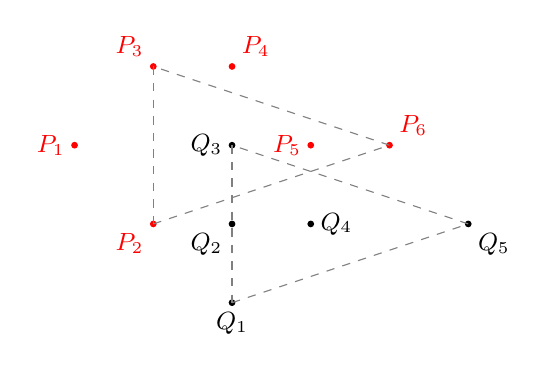
\begin{tikzpicture}
    \filldraw[red] (0, 2) circle (1pt) node[anchor=east]{\small $P_1$};
    \filldraw[red] (1, 1) circle (1pt) node[anchor=north east]{\small $P_2$};
    \filldraw[red] (1, 3) circle (1pt) node[anchor=south east]{\small $P_3$};
    \filldraw[red] (2, 3) circle (1pt) node[anchor=south west]{\small $P_4$};
    \filldraw[red] (3, 2) circle (1pt) node[anchor=east]{\small $P_5$};
    \filldraw[red] (4, 2) circle (1pt) node[anchor=south west]{\small $P_6$};
    \filldraw[black] (2, 0) circle (1pt) node[anchor=north]{\small $Q_1$};
    \filldraw[black] (2, 1) circle (1pt) node[anchor=north east]{\small $Q_2$};
    \filldraw[black] (2, 2) circle (1pt) node[anchor=east]{\small $Q_3$};
    \filldraw[black] (3, 1) circle (1pt) node[anchor=west]{\small $Q_4$};
    \filldraw[black] (5, 1) circle (1pt) node[anchor=north west]{\small $Q_5$};
    \draw[dashed, color=gray] (1, 1) -- (4, 2);
    \draw[dashed, color=gray] (4, 2) -- (1, 3);
    \draw[dashed, color=gray] (1, 3) -- (1, 1);
    \draw[dashed, color=gray] (2, 0) -- (5, 1);
    \draw[dashed, color=gray] (5, 1) -- (2, 2);
    \draw[dashed, color=gray] (2, 2) -- (2, 0);
  \end{tikzpicture}
\end{figure}

\subsection{輸入格式}

\begin{format}
\f{
$n$ $m$
$x_1$ $y_1$
$x_2$ $y_2$
$\vdots$
$x_n$ $y_n$
$\xi_1$ $\eta_1$
$\xi_2$ $\eta_2$
$\vdots$
$\xi_m$ $\eta_m$
}
\end{format}

\begin{itemize}
\tightlist
\item
  \(n\) 代表 \(S_1\) 的集合大小。
\item
  \(m\) 代表 \(S_2\) 的集合大小。
\item
  \(x_i, y_i\) 代表 \(S_1\) 包含點 \((x_i, y_i)\)。
\item
  \(\xi_i, \eta_i\) 代表 \(S_2\) 包含點 \((\xi_i, \eta_i)\)。
\end{itemize}

\subsection{輸出格式}

\begin{format}
\f{
$k$
$a_1$
$a_2$
$\vdots$
$a_k$
}
\end{format}

\begin{itemize}
\tightlist
\item
  \(k\) 代表若子凸包 \(\operatorname{Conv}(T_1)\) 與子凸包
  \(\operatorname{Conv}(T_2)\)
  經過平移後重合,\(\operatorname{Conv}(T_1)\) 所有可能的非 \(0\)
  面積數。
\item
  \(a_i\) 為一整數,代表 \(\operatorname{Conv}(T_1)\) 所有可能的非 \(0\)
  面積中,第 \(i\) 小的數的\textbf{兩倍}。
\end{itemize}

\subsection{測資限制}

\begin{itemize}
\tightlist
\item
  \(3 \le n \le 40\)。
\item
  \(3 \le m \le 40\)。
\item
  \(0 \le x_i \le 20\)。
\item
  \(0 \le y_i \le 20\)。
\item
  \(0 \le \xi_i \le 20\)。
\item
  \(0 \le \eta_i \le 20\)。
\item
  對任意 \(i, j \in \{1, 2, \ldots, n\}\),若 \(i \ne j\),則
  \((x_i, y_i) \ne (x_j, y_j)\)。
\item
  對任意 \(i, j \in \{1, 2, \ldots, m\}\),若 \(i \ne j\),則
  \((\xi_i, \eta_i) \ne (\xi_j, \eta_j)\)。
\item
  輸入的數皆為整數。
\end{itemize}

\subsection{範例測試}

\begin{example}
\exmp{
6 5
0 2
1 1
1 3
2 3
3 2
4 2
2 0
2 1
2 2
3 1
5 1
}{%
1
6
}%
\exmp{
4 4
0 0
1 1
1 2
2 0
2 0
1 2
1 1
0 0
}{%
3
1
2
4
}%
\exmp{
4 4
0 1
1 1
1 2
2 2
0 1
1 0
1 1
2 0
}{%
0
}%
\end{example}

\subsection{評分說明}

本題共有四組子任務,條件限制如下所示。
每一組可有一或多筆測試資料,該組所有測試資料皆需答對才會獲得該組分數。

\begin{longtable}[]{@{}ccl@{}}
\toprule
子任務 & 分數 & 額外輸入限制 \\
\midrule
\endhead
1 & \(7\) & 所有可能的非 \(0\) 面積必能從 \(T_1\) 與 \(T_2\) 中各選
\(3\) 個點得到 \\
2 & \(23\) & \(n+m \le 30\) \\
3 & \(41\) & \(S_1 = S_2\) \\
4 & \(29\) & 無額外限制 \\
\bottomrule
\end{longtable}

\section{迷宮鑰匙圈 (Maze)}

\subsection{問題描述}

小咪到夜市玩遊戲,贏得了一副鑰匙圈。這副鑰匙圈上有個迷宮面板,裡面有好幾顆小鋼珠:

\begin{figure}[!htb]
  \centering
  \includegraphics[width=0.5\linewidth]{maze1.jpg}
  \caption{圖片來源:FB 粉絲專頁「小藍貓 :3」(BlueCatFriends)}
\end{figure}

\noindent 將鑰匙圈的面板向左或向右旋轉 \(90\)
度,可以使每顆仍在迷宮內的小鋼珠向下掉落,直到該小鋼珠掉出迷宮,碰到迷宮擋板,或碰到其他仍在迷宮內的小鋼珠為止。更明確地說,這座迷宮可以用
\(N\times M\) 的二維矩陣表示,一次的 \(90\) 度旋轉會將迷宮變換為
\(M\times N\) 的二維矩陣,其中

\begin{itemize}
\tightlist
\item
  一次 \(90\) 度左旋轉會將位置 \((i, j)\) 變換成位置 \((M-j+1, i)\)。
\item
  一次 \(90\) 度右旋轉會將位置 \((i, j)\) 變換成位置 \((j, N-i+1)\)。
\end{itemize}

\noindent 此外,若旋轉後位置 \((i, j)\) 有一顆小鋼珠,則

\begin{itemize}
\tightlist
\item
  若存在某個 \(i' > i\) 滿足 \((i', j)\) 為迷宮擋板,則

  \begin{enumerate}
  \def\labelenumi{\arabic{enumi}.}
  \tightlist
  \item
    設最小的 \(i'\) 為 \(i^*\)。
  \item
    若 \((i, j), (i+1, j), \ldots, (i^*-1, j)\) 間恰有 \(k\)
    顆小鋼珠,則原位置 \((i, j)\) 的小鋼珠會掉到位置 \((i^*-k, j)\)。
  \end{enumerate}
\item
  否則,該小鋼珠將掉出迷宮。
\end{itemize}

給定迷宮與小鋼珠的起始位置,請算出至少需要向左或向右旋轉 \(90\)
度幾次,才能使每顆小鋼珠都掉出迷宮。

以下是一個迷宮大小為 \(10\times7\) 的例子:

\begin{figure}[h]
\centering
\includegraphics{maze2.png}
\caption{}
\end{figure}

\subsection{輸入格式}

\begin{format}
\f{
$n$ $m$
$s_{1, 1}$ $s_{1, 2}$ $\ldots$ $s_{1, m}$
$s_{2, 1}$ $s_{2, 2}$ $\ldots$ $s_{2, m}$
$\vdots$
$s_{n, 1}$ $s_{n, 2}$ $\ldots$ $s_{n, m}$
}
\end{format}

\begin{itemize}
\tightlist
\item
  \(n\) 代表迷宮的列數。
\item
  \(m\) 代表迷宮的行數。
\item
  \(s_{i, j}\) 代表位置 \((i, j)\) 的狀態,以字元
  \texttt{b}、\texttt{s}、\texttt{w} 表示,其中

  \begin{enumerate}
  \def\labelenumi{\arabic{enumi}.}
  \tightlist
  \item
    \texttt{b} 代表該格為空且有小鋼珠。
  \item
    \texttt{s} 代表該格為空且沒有小鋼珠。
  \item
    \texttt{w} 代表該格為迷宮擋板。
  \end{enumerate}
\end{itemize}

\subsection{輸出格式}

如果存在使每顆小鋼珠都掉出迷宮的旋轉方式,請輸出

\begin{format}
\f{
$\textrm{ans}$
}
\end{format}

\noindent 其中 \(\textrm{ans}\)
為一整數,代表所需的旋轉次數。否則,請輸出

\begin{format}
\f{
$-1$
}
\end{format}

\subsection{測資限制}

\begin{itemize}
\tightlist
\item
  \(1 \le n \le 15\)。
\item
  \(1 \le m \le 15\)。
\item
  對任意 \(i \in \{1, 2, \ldots, n\}\) 與
  \(j \in \{1, 2, \ldots, m\}\),\(s_{i, j}\) 只能是
  \texttt{b}、\texttt{s}、或 \texttt{w}。
\item
  滿足 \(s_{i, j}\) 為 \texttt{b} 的 \((i, j)\) 對數介於 \(1\) 與 \(3\)
  之間。
\item
  給定的迷宮保證不會有不穩定的狀態,亦即若 \(s_{i, j}\) 為
  \texttt{b},則必定存在某個 \(i^* > i\) 滿足

  \begin{enumerate}
  \def\labelenumi{\arabic{enumi}.}
  \tightlist
  \item
    \(s_{i^*, j}\) 為 \texttt{w}。
  \item
    \(s_{i, j}, s_{i+1, j}, \ldots, s_{i^*-1, j}\) 均為 \texttt{b}。
  \end{enumerate}
\item
  \(n\) 與 \(m\) 皆為整數。
\end{itemize}

\subsection{範例測試}

\begin{example}
\exmp{
10 7
w w w w w w w
w s s s s s w
w s s s s s w
w s w w w s w
w s s s w s w
w s b b w s w
w w w w w s w
s s s s s s w
s s s s s s w
w w w w w w w
}{%
7
}%
\exmp{
5 3
s w s
s s s
w b w
w b w
s w s
}{%
5
}%
\exmp{
5 3
s w s
w s w
s b s
w b w
s w s
}{%
-1
}%
\end{example}

\subsection{評分說明}

本題共有三組子任務,條件限制如下所示。
每一組可有一或多筆測試資料,該組所有測試資料皆需答對才會獲得該組分數。

\begin{longtable}[]{@{}ccl@{}}
\toprule
子任務 & 分數 & 額外輸入限制 \\
\midrule
\endhead
1 & \(37\) & 迷宮裡的小鋼珠數量為 \(1\) \\
2 & \(29\) & 迷宮裡的小鋼珠數量不超過 \(2\) \\
3 & \(34\) & 無額外限制 \\
\bottomrule
\end{longtable}

\section{恐怖的黑色魔物 (Monster)}

\subsection{問題描述}

G
公司最近用黑科技在某個神秘的地方建立了新的研發總部。這座研發總部的形狀是個長方體,內部共有
\(F\) 層樓,每一層樓均有形狀大小相同且由 \(M\) 列 \(N\)
行組成的矩形房間。一個房間的位置以三個正整數 \((p, q, r)\)
表示,代表該房間位於研發總部 \(p\) 樓的第 \(q\) 列第 \(r\) 行。

G
公司的員工均可以透過黑科技直接傳送至隔壁、樓下或樓上的房間。更明確地說,位於房間
\((p, q, r)\) 的 G 公司員工,

\begin{enumerate}
\def\labelenumi{\arabic{enumi}.}
\tightlist
\item
  當 \(p > 1\) 時,可傳送至房間 \((p-1, q, r)\)。
\item
  當 \(p < F\) 時,可傳送至房間 \((p+1, q, r)\)。
\item
  當 \(q > 1\) 時,可傳送至房間 \((p, q-1, r)\)。
\item
  當 \(q < M\) 時,可傳送至房間 \((p, q+1, r)\)。
\item
  當 \(r > 1\) 時,可傳送至房間 \((p, q, r-1)\)。
\item
  當 \(r < N\) 時,可傳送至房間 \((p, q, r+1)\)。
\end{enumerate}

G 公司為了節省員工的用餐休息時間,在其中的 \(R\)
個房間開設了餐廳,方便員工在研發總部內直接用餐。但餐廳的食物會滋生一種恐怖的黑色魔物,有一部分的
G 公司員工非常害怕這種恐怖的黑色魔物,因此不敢在這些餐廳用餐。

你的上司 K
先生特別害怕這種恐怖的黑色魔物。他總認為這些恐怖的黑色魔物,也能透過黑科技,在研發總部裡自由穿梭。他定義了「黑色恐怖距離」:若一個房間至少須使用
\(d\) 次黑科技傳送,才能抵達餐廳,則該房間的黑色恐怖距離就是 \(d\)。對 K
先生來說,黑色恐怖距離越小就越恐怖,因次他每次在研發總部內移動時,都會計算該如何使用黑科技,才能讓途中經過的房間,最小的黑色恐怖距離最大。作為
K 先生下屬的你,打算撰寫一個程式,幫助 K
先生快速算出在最不恐怖的路徑上,所經過的房間裡黑色恐怖距離的最小值。

\subsection{輸入格式}

\begin{format}
\f{
$F$ $M$ $N$
$R$
$p_1$ $q_1$ $r_1$
$p_2$ $q_2$ $r_2$
$\vdots$
$p_R$ $q_R$ $r_R$
$Q$
$a_1$ $b_1$ $c_1$ $x_1$ $y_1$ $z_1$
$a_2$ $b_2$ $c_2$ $x_2$ $y_2$ $z_2$
$\vdots$
$a_Q$ $b_Q$ $c_Q$ $x_Q$ $y_Q$ $z_Q$
}
\end{format}

\begin{itemize}
\tightlist
\item
  \(F\) 代表 G 公司研發總部的樓層數。
\item
  \(M\) 代表 G 公司研發總部的列數。
\item
  \(N\) 代表 G 公司研發總部的行數。
\item
  \(R\) 代表 G 公司研發總部的餐廳數。
\item
  \((p_i, q_i, r_i)\) 代表 G 公司研發總部內第 \(i\) 間餐廳的位置。
\item
  \(Q\) 代表 K 先生計畫移動的次數。
\item
  \((a_i, b_i, c_i)\) 代表 K 先生計畫第 \(i\) 次移動的起點。
\item
  \((x_i, y_i, z_i)\) 代表 K 先生計畫第 \(i\) 次移動的終點。
\end{itemize}

\subsection{輸出格式}

\begin{format}
\f{
$d_1^*$
$d_2^*$
$\vdots$
$d_Q^*$
}
\end{format}

\begin{itemize}
\tightlist
\item
  \(d_i^*\) 代表 K 先生第 \(i\)
  次移動時,所有可能的路徑中,最小黑色恐怖距離的最大值。
\end{itemize}

\subsection{測資限制}

\begin{itemize}
\tightlist
\item
  \(1 \le F \le 2\times10^5\)。
\item
  \(1 \le M \le 2\times10^5\)。
\item
  \(1 \le N \le 2\times10^5\)。
\item
  \(1 \le FMN \le 2\times10^5\)。
\item
  \(1 \le R \le FMN\)。
\item
  \(1 \le p_i \le F\)。
\item
  \(1 \le q_i \le M\)。
\item
  \(1 \le r_i \le N\)。
\item
  \(1 \le Q \le 2\times10^5\)。
\item
  \(1 \le a_i \le F\)。
\item
  \(1 \le b_i \le M\)。
\item
  \(1 \le c_i \le N\)。
\item
  \(1 \le x_i \le F\)。
\item
  \(1 \le y_i \le M\)。
\item
  \(1 \le z_i \le N\)。
\item
  對任意 \(i, j \in \{1, 2, \ldots, R\}\),若 \(i \ne j\),則
  \((p_i, q_i, r_i) \ne (p_j, q_j, r_j)\)。
\item
  輸入的數皆為整數。
\end{itemize}

\subsection{範例測試}

\begin{example}
\exmp{
3 3 3
3
1 1 1
2 2 2
3 3 3
4
1 3 3 3 1 1
1 2 2 3 2 2
1 2 3 1 2 3
1 1 1 3 3 3
}{%
2
1
2
0
}%
\exmp{
1 1 3
1
1 1 2
1
1 1 1 1 1 3
}{%
0
}%
\end{example}

\subsection{評分說明}

本題共有五組子任務,條件限制如下所示。
每一組可有一或多筆測試資料,該組所有測試資料皆需答對才會獲得該組分數。

\begin{longtable}[]{@{}ccl@{}}
\toprule
子任務 & 分數 & 額外輸入限制 \\
\midrule
\endhead
1 & \(6\) & \(F = R = 1, MN \le 100, Q \le 100\) \\
2 & \(21\) & 對任意 \(i \in \{1, 2, \ldots, Q\}\),均有
\((a_i, b_i, c_i) = (x_i, y_i, z_i)\) \\
3 & \(4\) & \(FMN \le 3000\) \\
4 & \(25\) & \(Q = 1\) \\
5 & \(44\) & 無額外限制 \\
\bottomrule
\end{longtable}

\section{博物館 (Museum)}

\subsection{問題描述}

在 H 國有一座博物館,陳列了 \(n\)
件作品在一條直線的走廊上。從門口開始,由左至右,放置於第 \(i\)
個位置的作品價值為 \(c_i\)。

今日有重要的貴賓要蒞臨博物館,但是因為行程緊湊,貴賓只能觀賞最接近門口,也就是最左邊的
\(k\)
件作品。為了提升博物館的形象,博物館館長打算把一些貴重的作品移至前方。亦即把價值最高的前
\(k\) 件作品移至最左邊的 \(k\) 個位置。

因為博物館中的作品都非常地珍貴,每一次搬動,都只能交換相鄰的兩件作品,並且為了最小化損壞作品的風險,館長要求要用最少次數的搬動來完成。

給定當前每件作品的價值,請輸出最少的搬動次數以完成館長的要求。

\subsection{輸入格式}

\begin{format}
\f{
$n$ $k$
$c_1$ $c_2$ $\dots$ $c_n$
}
\end{format}

\begin{itemize}
\tightlist
\item
  \(n\) 表示作品的數量。
\item
  \(k\) 表示貴賓欣賞的作品數量。
\item
  \(c_i\) 表示當前放置於第 \(i\) 個位置的作品價值。
\end{itemize}

\subsection{輸出格式}

\begin{format}
\f{
$m$
}
\end{format}

\begin{itemize}
\tightlist
\item
  \(m\) 為滿足館長要求的最少搬動次數。
\end{itemize}

\subsection{測資限制}

\begin{itemize}
\tightlist
\item
  \(1 \le k \le n \le 10^5\)。
\item
  \(1 \le c_i\le 10^{9}\)。
\item
  輸入的數皆為整數。
\end{itemize}

\subsection{範例測試}

\begin{example}
\exmp{
5 3
1 2 3 4 5
}{%
6
}%
\exmp{
6 2
2 3 2 3 2 3
}{%
3
}%
\end{example}

\subsection{評分說明}

本題共有三組子任務,條件限制如下所示。
每一組可有一或多筆測試資料,該組所有測試資料皆需答對才會獲得該組分數。

\begin{longtable}[]{@{}ccl@{}}
\toprule
子任務 & 分數 & 額外輸入限制 \\
\midrule
\endhead
1 & \(3\) & \(n \le 500\) 且 \(c_1, c_2, \ldots, c_n\) 兩兩相異 \\
2 & \(19\) & \(c_1, c_2, \ldots, c_n\) 兩兩相異 \\
3 & \(78\) & 無額外限制 \\
\bottomrule
\end{longtable}

\section{整數的迴文分解法 (Palindrome)}

\subsection{問題描述}

H
教授是一位密碼學專家,他現在正在研究如何對一個正整數做特殊分解,因而發明了正整數的迴文分解法,其分解方法如下:對於一個正整數
\(n\),把 \(n\) 分解成 \(k\) 個正整數 \(x_1, x_2, \ldots, x_k\)
的和,滿足 \(n = x_1 + x_2 + \ldots + x_k\),且
\(x_1, x_2, \ldots, x_k\) 由左讀到右和由右讀到左相同。

當兩種分解法分解出來的正整數數量不同,或是出現的次序不同時,則視為不同的分解法。更嚴謹地說,設
\(n = a_1 + a_2 + \ldots + a_k = b_1 + b_2 + \ldots + b_l\)
為兩種迴文分解法。若 \(k \ne l\),或者 \(k = l\) 但存在
\(i \in \{1, 2, \ldots, k\}\) 使得
\(a_i \ne b_i\),則視為不同的分解法。例如正整數 \(6\) 有 \(8\)
種迴文分解法,分別是

\begin{enumerate}
\def\labelenumi{\arabic{enumi}.}
\tightlist
\item
  \(6\);
\item
  \(2 + 2 + 2\);
\item
  \(3 + 3\);
\item
  \(2 + 1 + 1 + 2\);
\item
  \(1 + 4 + 1\);
\item
  \(1 + 1 + 2 + 1 + 1\);
\item
  \(1 + 2 + 2 + 1\);
\item
  \(1 + 1 + 1 + 1 + 1 + 1\)。
\end{enumerate}

給定一個正整數 \(n\),請寫一支電腦程式去計算 \(n\)
有多少種不同的迴文分解法。因為這個數字可能很大,你只要求出方法數除以
\(10^9 + 7\) 的餘數就行了。

\subsection{輸入格式}

\begin{format}
\f{
$t$
$n_1$
$n_2$
\vdots
$n_t$
}
\end{format}

\begin{itemize}
\tightlist
\item
  \(t\) 代表你的電腦程式需要處理的正整數 \(n\) 的個數。
\item
  \(n_i\) 代表第 \(i\) 筆詢問的正整數 \(n\)。
\end{itemize}

\subsection{輸出格式}

\begin{format}
\f{
$\textrm{ans}_1$
$\textrm{ans}_2$
\vdots
$\textrm{ans}_t$
}
\end{format}

\begin{itemize}
\tightlist
\item
  \(\textrm{ans}_i\) 代表 \(n_i\) 的迴文分解方法數除以 \(10^9 + 7\)
  的餘數。
\end{itemize}

\subsection{測資限制}

\begin{itemize}
\tightlist
\item
  \(1 \le t \le 10^4\)。
\item
  \(1 \le n_i \le 10^{15}\)。
\item
  輸入的數皆為整數。
\end{itemize}

\subsection{範例測試}

\begin{example}
\exmp{
2
3
6
}{%
2
8
}%
\end{example}

\subsection{評分說明}

本題共有四組子任務,條件限制如下所示。
每一組可有一或多筆測試資料,該組所有測試資料皆需答對才會獲得該組分數。

\begin{longtable}[]{@{}ccl@{}}
\toprule
子任務 & 分數 & 額外輸入限制 \\
\midrule
\endhead
1 & \(10\) & 輸入的 \(n_i\) 兩兩相異,且 \(n_i \le 30\) \\
2 & \(30\) & \(n_i \le 1000\) \\
3 & \(10\) & \(n_i \le 10^6\) \\
4 & \(50\) & 無額外限制 \\
\bottomrule
\end{longtable}

\section{對戰機器馬 (Race)}

\subsection{問題描述}

這天,小齊與小田各派出 \(n\) 隻機器馬進行 \(n\)
回一對一的對戰,雙方的出賽順序均已排定且不得再更改。已知對於
\(1\le i \le n\),小齊第 \(i\) 場出賽的機器馬原始戰力是 \(a_i\),小田第
\(i\) 場的機器馬原始戰力則是 \(b_i\),且 \(0\le a_i, b_i< P\),其中
\(P\) 是一個給定的正整數。每一場對戰時,戰力高者獲勝。

小田為了贏取更多的勝利,研發出了能調整這些機器馬戰力的燃料,每一種燃料有一個魔力值
\(m\),當原始戰力 \(b_i\) 的機器馬使用了魔力值 \(m\)
的燃料,戰力就會變成 \((b_i + m) \% P\),這裡 \(\%\)
表示取餘數的運算。對小田來說,如果每一隻機器馬都可以挑選不同魔力值的燃料,當然就太好了,但是由於某些限制,小田只能生產出最多兩種燃料,且每一隻機器馬都必須使用恰一種燃料才可以。換句話說,小田可以選擇兩個非負整數
\(s\) 與 \(t\),若 \((b_i + s) \% P > a_i\) 或
\((b_i + t) \% P > a_i\),則小田可以贏得第 \(i\)
場比賽的勝利。小田希望能挑選出兩種魔力值,以獲得最多的勝利。請計算並輸出小田的最大勝利場次數。請注意,小田的每一隻機器馬必須使用所生產的兩種燃料之一,即使原先戰力已經勝過對方的機器馬也必須挑選其中之一使用。

舉例來說,假設
\(P=10\),小齊與小田的原始戰力如下表。若小田選擇生產魔力值 \(s=1\) 與
\(t=6\) 的兩種燃料,那麼他可以戰勝 \(5\) 場比賽。另,小田沒有戰勝 \(6\)
場以上比賽的可能,因此所求答案是 \(5\)。

\begin{center}
\begin{tabular}{|l|l|l|l|l|l|l|l|}
\hline
小齊戰力 $a_i$ & $6$ & $7$ & $9$ & $4$ & $8$ & $5$ & $5$ \\
\hline
小田戰力 $b_i$ & $3$ & $7$ & $6$ & $9$ & $9$ & $1$ & $5$ \\
\hline
$s=1$ 與 $t=6$ & $3 + 6 > 6$ & $7 + 1 > 7$ & & $(9 + 6) \% 10 > 4$ & & $1 + 6 > 5$ & $5 + 1 > 5$ \\
\hline
\end{tabular}
\end{center}

\subsection{輸入格式}

\begin{format}
\f{
$n$ $P$
$a_1$ $a_2$ $\ldots$ $a_n$
$b_1$ $b_2$ $\ldots$ $b_n$
}
\end{format}

\begin{itemize}
\tightlist
\item
  \(n\) 代表比賽的回合數,同時也是小齊和小田各自派出的機器馬數量。
\item
  \(P\) 代表計算戰力用的參數。
\item
  \(a_i\) 代表小齊第 \(i\) 場出賽的機器馬原始戰力。
\item
  \(b_i\) 代表小田第 \(i\) 場出賽的機器馬原始戰力。
\end{itemize}

\subsection{輸出格式}

\begin{format}
\f{
$\textrm{ans}$
}
\end{format}

\begin{itemize}
\tightlist
\item
  \(\textrm{ans}\) 代表小田的最大勝利場次數。
\end{itemize}

\subsection{測資限制}

\begin{itemize}
\tightlist
\item
  \(1 \le n \le 2\times 10^5\)。
\item
  \(1 \le P \le 10^9\)。
\item
  \(0 \le a_i < P\)。
\item
  \(0 \le b_i < P\)。
\item
  輸入的數皆為整數。
\end{itemize}

\subsection{範例測試}

\begin{example}
\exmp{
5 6
3 1 5 3 4
0 2 3 4 0
}{%
4
}%
\exmp{
7 10
6 7 9 4 8 5 5
3 7 6 9 9 1 5
}{%
5
}%
\end{example}

\subsection{評分說明}

本題共有五組子任務,條件限制如下所示。
每一組可有一或多筆測試資料,該組所有測試資料皆需答對才會獲得該組分數。

\begin{longtable}[]{@{}ccl@{}}
\toprule
子任務 & 分數 & 額外輸入限制 \\
\midrule
\endhead
1 & \(5\) & \(n \le 100, P \le 100\) \\
2 & \(7\) & \(n \le 100, P \le 10000\) \\
3 & \(17\) & \(n \le 5000\) \\
4 & \(40\) & 對於所有 \(i\),\(b_i \le a_i\) \\
5 & \(31\) & 無額外限制 \\
\bottomrule
\end{longtable}
